\documentclass{beamer}

\usepackage[utf8]{inputenc}
\usecolortheme{beaver}
\usepackage{caption}
\usepackage{subcaption}
\usepackage{mathtools}
\usepackage{todonotes}
\usepackage{amsmath}
\usepackage{bm}
\usepackage{listings}
\usepackage{ragged2e}
\usepackage{titlecaps}
\usepackage{fancyvrb}

\def\ci{\perp\!\!\!\!\!\perp}

\newtheorem{proposition}{Proposition}
\Addlcwords{for a is but and with of in as the etc on to if}

\setbeamertemplate{section in toc}{\inserttocsectionnumber.~\inserttocsection}
\usetheme{Boadilla}
\makeatletter
\setbeamertemplate{footline}{%
    \leavevmode%
    \hbox{%
        \begin{beamercolorbox}[wd=.3\paperwidth,ht=2.25ex,dp=1ex,center]{author in head/foot}%
            \usebeamerfont{author in head/foot}\insertshortauthor\expandafter\beamer@ifempty\expandafter{\beamer@shortinstitute}{}{~~(\insertshortinstitute)}
        \end{beamercolorbox}%
        \begin{beamercolorbox}[wd=.55\paperwidth,ht=2.25ex,dp=1ex,center]{title in head/foot}%
            \usebeamerfont{title in head/foot}\insertshorttitle
        \end{beamercolorbox}%
        \begin{beamercolorbox}[wd=.15\paperwidth,ht=2.25ex,dp=1ex,right]{date in head/foot}%
            \usebeamerfont{date in head/foot}\insertshortdate{}\hspace*{2em}
            \insertframenumber{} / \inserttotalframenumber\hspace*{2ex} 
        \end{beamercolorbox}}%
        \vskip0pt%
    }
\makeatother

\begin{document}

\title[]{A cautious approach to constraint-based causal model selection}
\date{}

\begin{frame}
	\begin{figure}
		
\includegraphics[scale=0.3]{imgs/title.png}
	\end{figure}
\end{frame}

\begin{frame}{DAGs and Implied Conditional Independences}
	Each missing edge implies a Conditional Independence (CI) statement.

	\begin{figure}
		\centering
		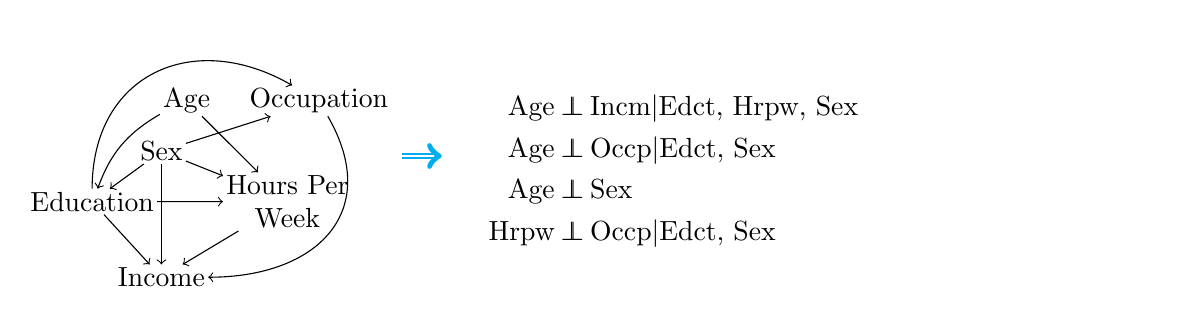
\begin{tikzpicture}
			\begin{scope}[yshift=0.7cm, scale=0.8]
			\tikzstyle{every node}=[align=center, inner sep=1pt]
				\node (sex) at (-0.7, -0.8) {Sex};
				\node (age) at (-0.3, 0) {Age};
				\node (ed) at (-1.8, -1.6) {Education};
				\node (occ) at (1.8, 0) {Occupation};
				\node (hrpw) at (1.3, -1.6) {Hours Per \\ Week};
				\node (income) at (-0.7, -2.8) {Income};
			
				\draw[->]  (age) to[bend right=20] (ed);
				\draw[->]  (sex) to (ed);
				\draw[->]  (age) to (hrpw);
				\draw[->]  (ed) to (hrpw);
				\draw[->]  (sex) to (hrpw);
				\draw[->]  (ed) to (income);
				\draw[->]  (hrpw) to (income);
				\draw[->]  (occ) to[out=300, in=0, looseness=1.4] (income.east);
				\draw[->]  (sex) to (income);
				\draw[->]  (ed) to[out=90, in=150, looseness=1.3] (occ);
				\draw[->]  (sex) to (occ);	
			\end{scope}
			\draw[thick, ->, double, cyan] (2.5,0) -- (3,0);
			\node[rectangle, align=center, inner sep=1pt] at (6, 0) {
				\begin{minipage}{\textwidth}
					\begin{equation*}
						\begin{split}
							\textnormal{Age} &\ci \textnormal{Incm} \rvert \textnormal{Edct, Hrpw, Sex} \\
							\textnormal{Age} &\ci \textnormal{Occp} \rvert \textnormal{Edct, Sex} \\
							\textnormal{Age} &\ci \textnormal{Sex} \\
							\textnormal{Hrpw} &\ci \textnormal{Occp} \rvert \textnormal{Edct, Sex} \\
						\end{split}
					\end{equation*}
				\end{minipage}
				};
		\end{tikzpicture}
	\end{figure}
	\vspace{1em}
	Datasets generated from this DAG should also satisfy these CIs (faithfulness).

\end{frame}

\begin{frame}{Constraint-Based Structure Learning}
	\center Constraint-based algorithms utilize CIs in data to learn DAGs.
	%\begin{figure}
	%	\centering
	%	\begin{tikzpicture}
	%		\begin{scope}
	%			\tikzstyle{every node}=[align=center, inner sep=1pt]
	%			\node (x1) at (0, 0) {$ X_1 $};
	%			\node (x2) at (0, -1) {$ X_2 $};
	%			\node (x3) at (1, -1) {$ X_3 $};
	%			\node (x4) at (1, 0) {$ X_4 $};

	%			\draw[->] (x1) to (x3);
	%			\draw[->] (x2) to (x3);
	%			\draw[->] (x3) to (x4);
	%		\end{scope}
	%		\begin{scope}[xshift=2cm]
	%			\draw[->] (0, -0.5) to (1, -0.5);
	%		\end{scope}
	%	\end{tikzpicture}
	%\end{figure}
	\begin{figure}
		\centering
		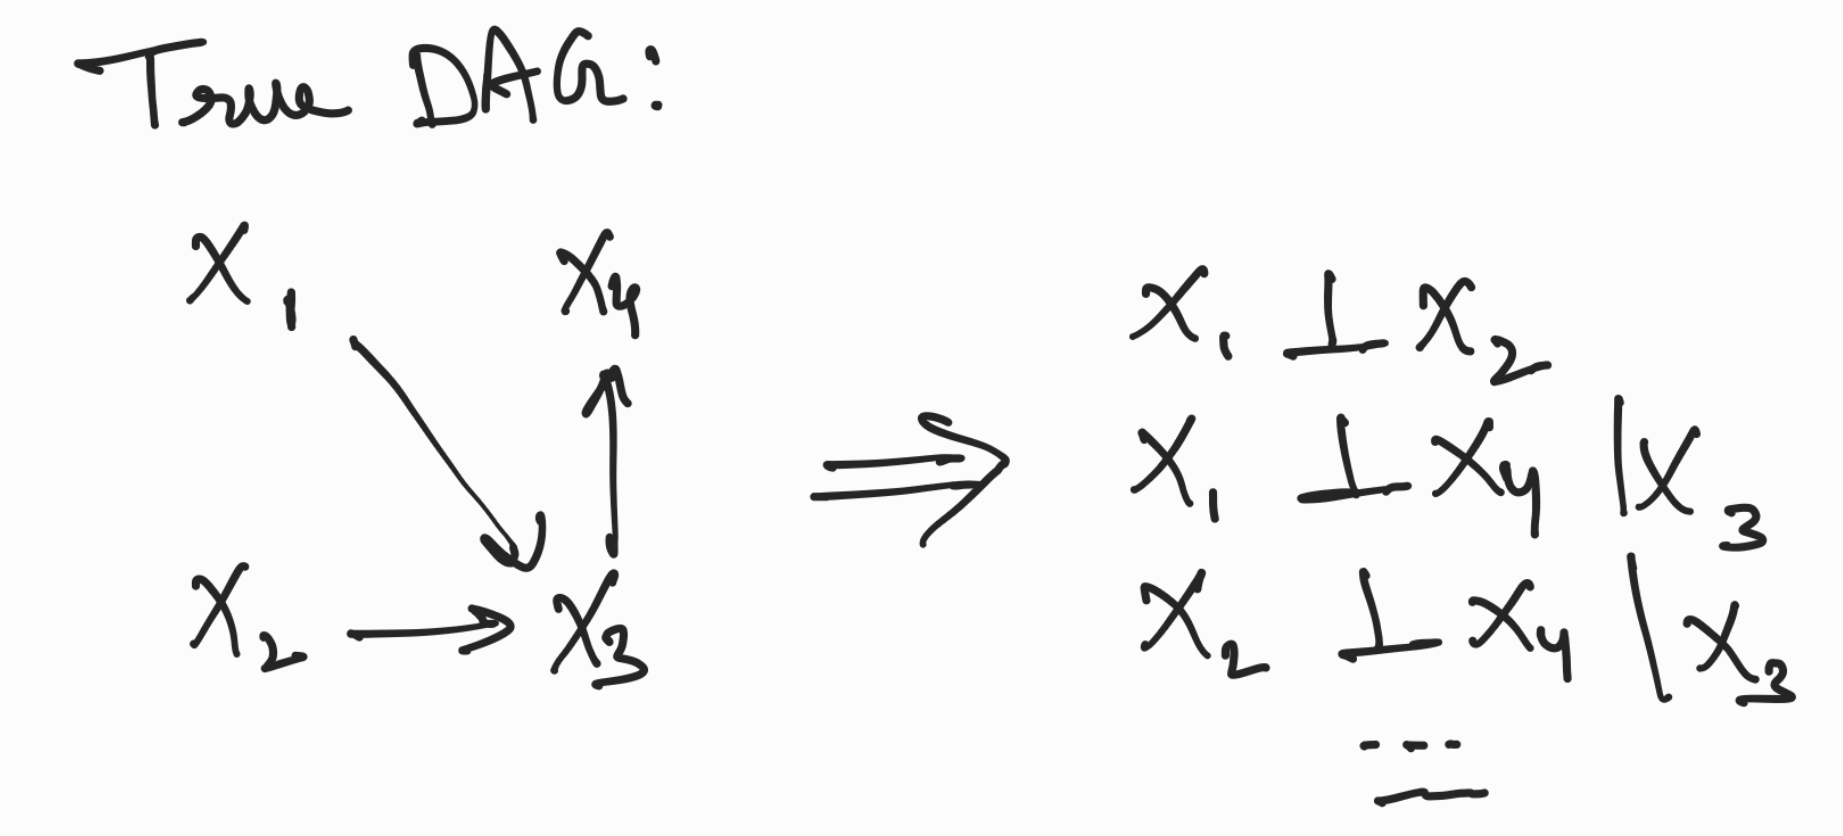
\includegraphics[scale=0.12]{imgs/example1.png}
	\end{figure}
	\begin{figure}
		\centering
		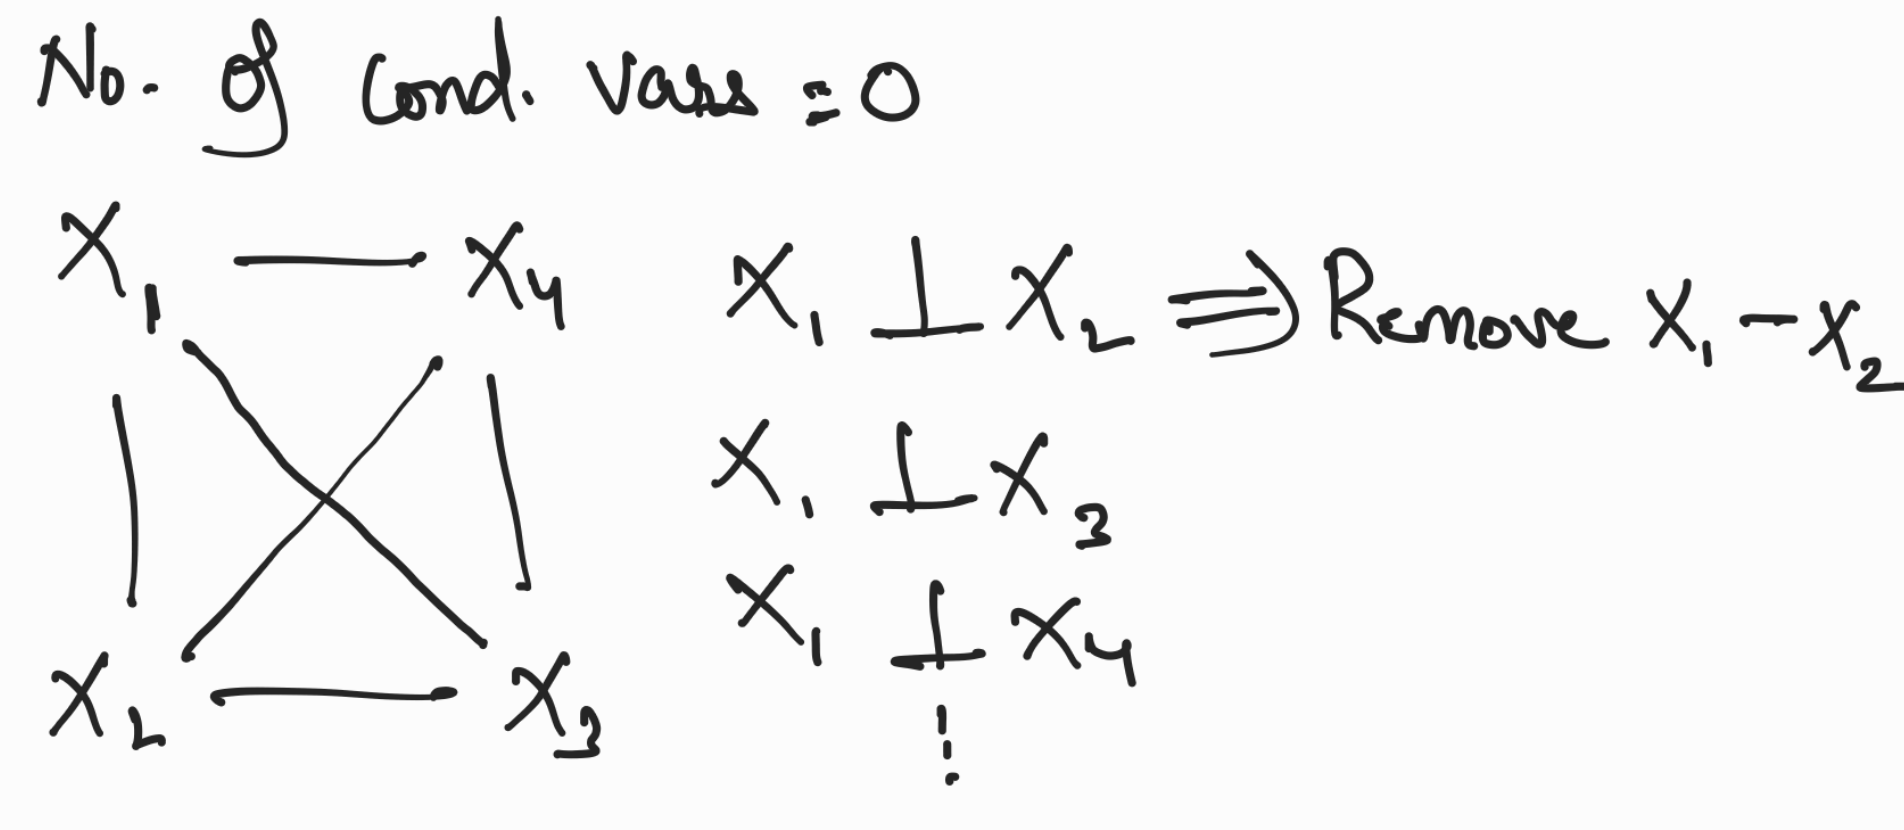
\includegraphics[scale=0.12]{imgs/example2.png}
	\end{figure}
\end{frame}

\begin{frame}
	\begin{figure}
		\centering
		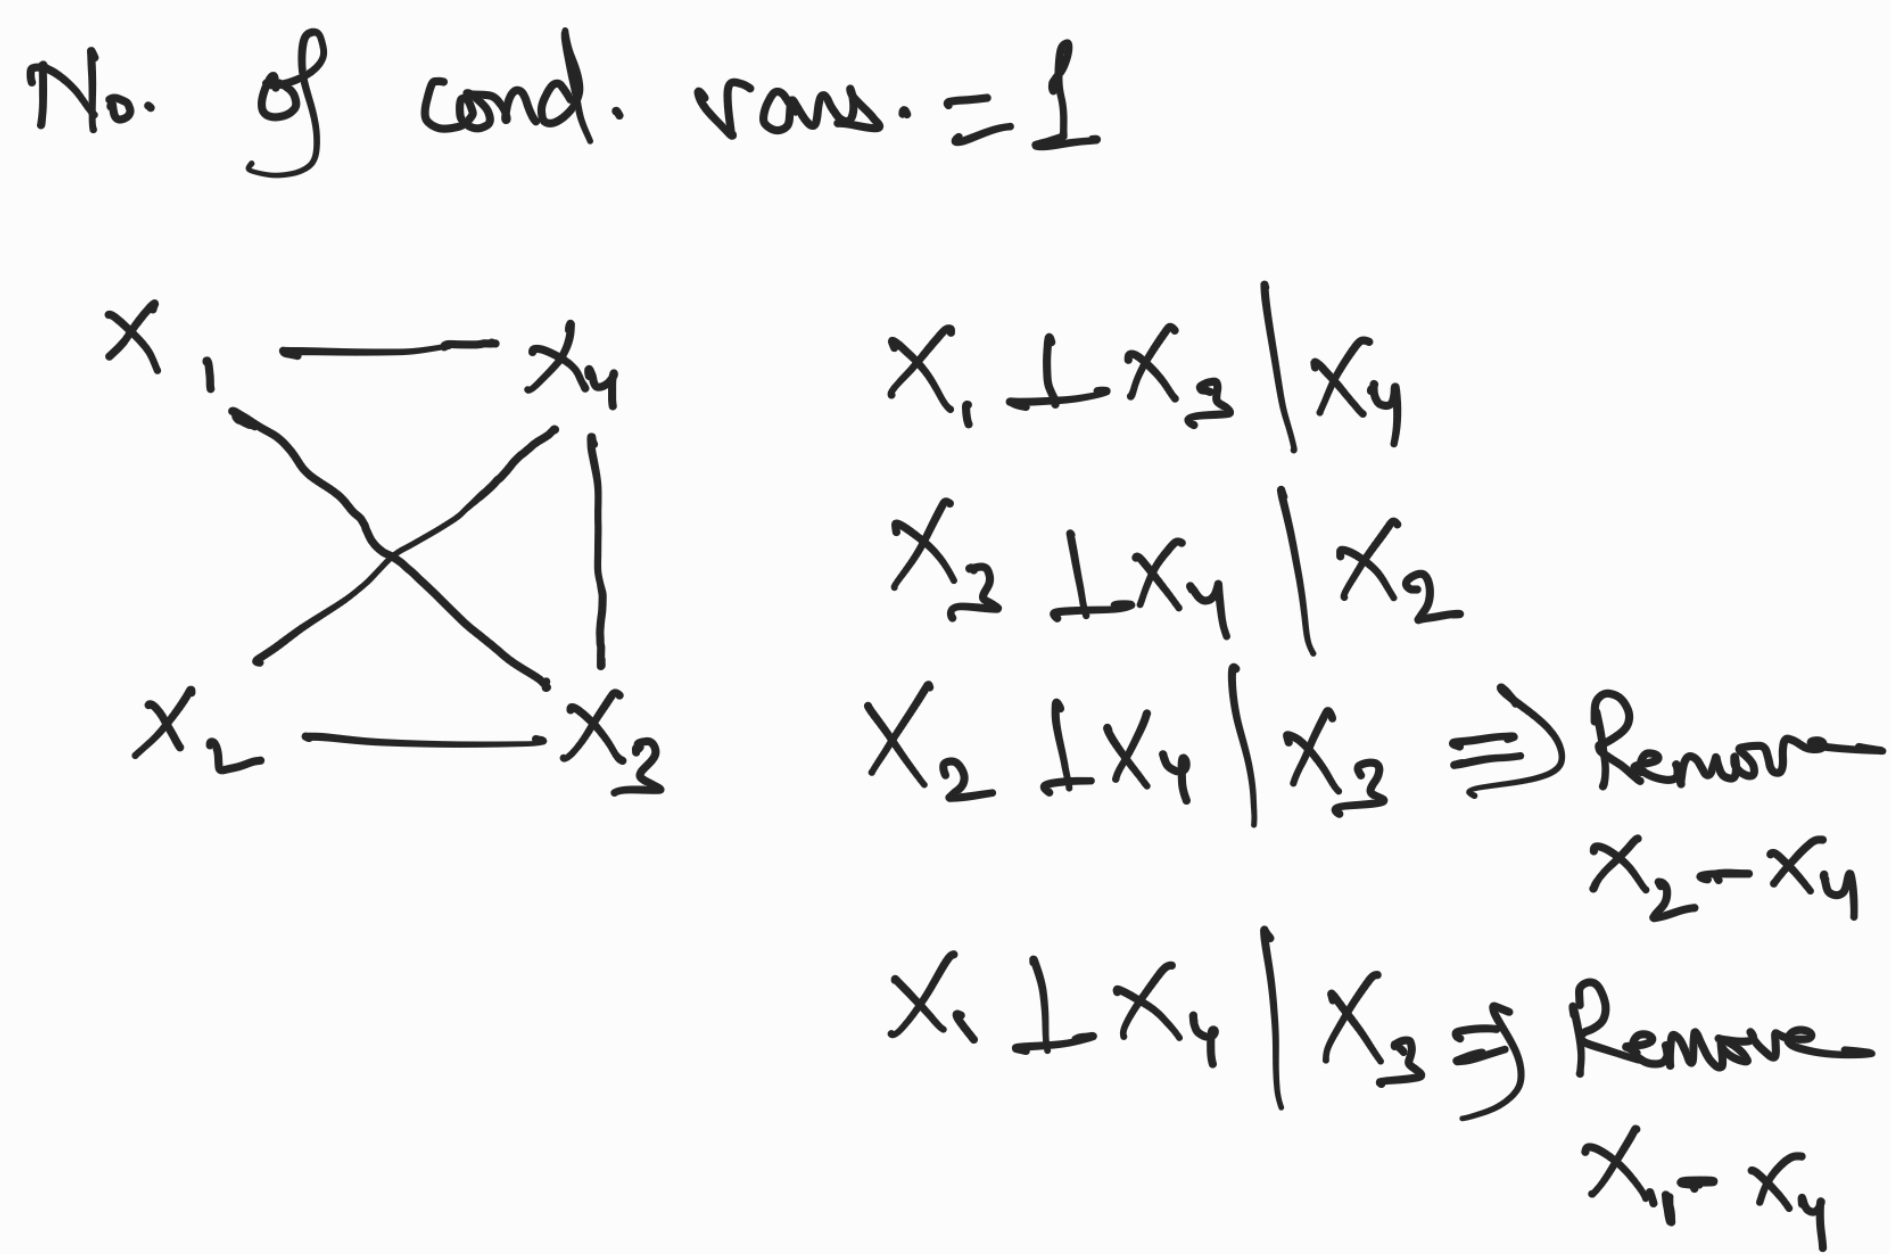
\includegraphics[scale=0.1]{imgs/example3.png}
	\end{figure}
	\begin{figure}
		\centering
		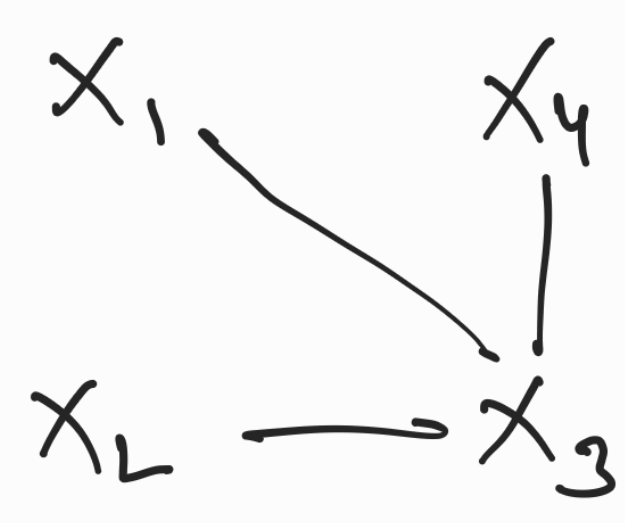
\includegraphics[scale=0.1]{imgs/example4.png}
	\end{figure}

	\center Edges are then oriented using Meek's rule.
\end{frame}

\begin{frame}{CI Testing in Data}
	Statistical tests are used to test CIs in data. Typically,
	\begin{equation*}
		\begin{split}
			H_0 &: X \ci Y \rvert Z \\
			H_A &: X \not \ci Y \rvert Z
		\end{split}
	\end{equation*}
	\vspace{2em}
	\center (p-value $ > \alpha $ ) $ \implies X \ci Y \rvert Z  \implies $ Remove Edge
\end{frame}

\begin{frame}{Problems With This Testing Approach}
	\begin{itemize}
		\item Has a tendency to estimate sparse structures, i.e., missing too many edges compared to ground truth.
		\item Methods focusing on controlling false positives (i.e., false edge inclusion) have been developed such as multiple testing adjustment.
		\item In practice, easy to achieve very few false edge inclusion, i.e., high precision.
		\item But difficult to achieve low rates of error for false edge exclusions, i.e., high recall.
		\item For downstream tasks, such as causal effect estimation, bias is largely driven by high rates of wrongly excluded edges.
	\end{itemize}
\end{frame}

\begin{frame}{Two Contexts For Structure Learning}
	\begin{itemize}
		\item \textbf{Causal Discovery:} Sparse models are better.
			\begin{itemize}
				\item Goal is to identify strong, novel, and promising causal relationships.
				\item Use the learned structure to plan possible experiments, or identify the most promising targets of intervention.
				\item E.g., high-dimensional genetics research, where the goal is to identify a small number of important genes that are promising targets.
				\item Precision is important.
			\end{itemize}
		\item \textbf{Submodel Selection:} Denser models are better.
			\begin{itemize}
				\item Goal is to quantify the effect of a small number of causal relationships of interest.
				\item Need to select a DAG that can be informative about strategies for identification or estimation.
				\item E.g., epidemiological settings where we are interested in estimating effects such as smoking on lung cancer.
				\item Recall is important.
			\end{itemize}
	\end{itemize}
\end{frame}

% \begin{frame}{Denser Models for Epidemiological Setting}
% 	\begin{itemize}
% 		\item Moderate-dimensional setting, more than $ 4 $ variables but less than hundreds.
% 		\item Causal graph could be partially known.
% 		\item Sparsity should not be assumed.
% 	\end{itemize}
% \end{frame}

\begin{frame}{Adjustment Sets From Denser Graph}
	\begin{figure}
		\centering
		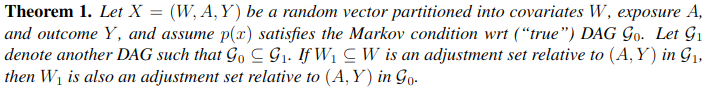
\includegraphics[scale=0.4]{imgs/theorem1.png}
	\end{figure}
	\begin{itemize}
		\item Using a super-DAG of the true DAG to select an adjustment set will always be valid.
	\end{itemize}
	\vspace{1em}
	\begin{figure}
		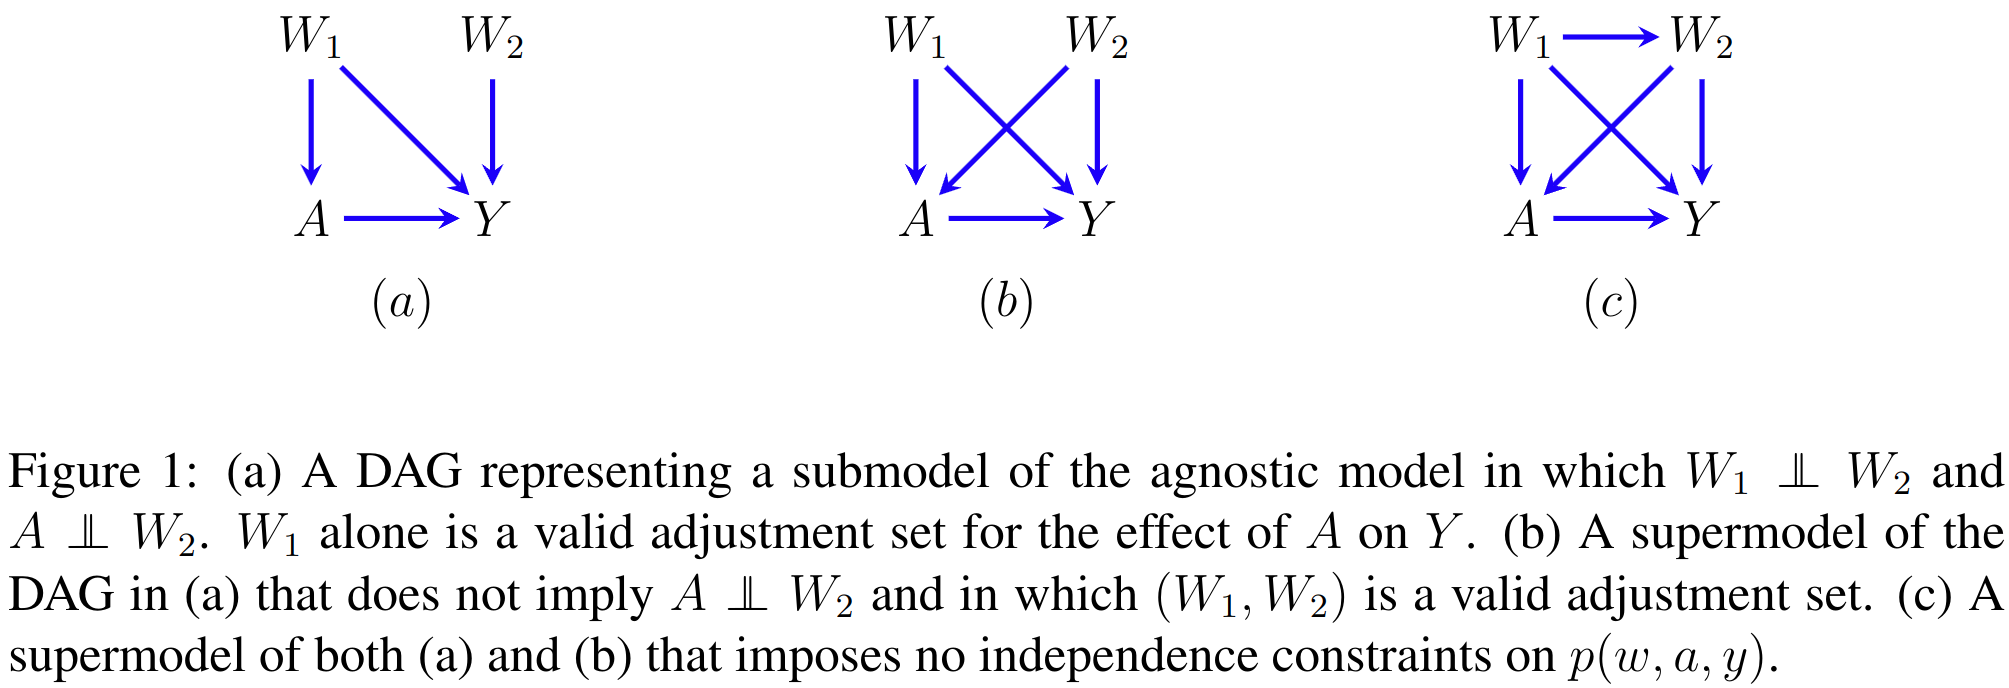
\includegraphics[scale=0.15]{imgs/figure1.png}
	\end{figure}
\end{frame}

\begin{frame}{Reformulating CI Test Hypothesis}
	\begin{itemize}
		\item $ \theta_{ij.S} $: Some measure of association between $ X_i $ and $ X_j $ given $ X_S $.
		\item $ \delta $: User chosen threshold.
	\end{itemize}

	\begin{equation*}
		\begin{split}
			H_0&: \rvert \theta_{ij.S} \rvert \ge \delta \\
			H_A&: \rvert \theta_{ij.S} \rvert < \delta \\
		\end{split}
	\end{equation*}

	\begin{itemize}
		\item $ H_0 $ implies dependence.
		\item Remove edge when $ H_0 $ is rejected.
	\end{itemize}
\end{frame}

\begin{frame}{Test Using Partial Correlation}
	\center When variables are multivariate Gaussian, Pearson's partial correlation.
	\vspace{1em}
	\begin{equation*}
		\begin{split}
			H_0&: \rvert \rho_{ij.S} \rvert \ge \delta \\
			H_A&: \rvert \rho_{ij.S} \rvert < \delta \\
		\end{split}
	\end{equation*}

	\begin{equation*}
		\begin{split}
			\textnormal{Fisher's z-transform: }& z(\hat{\rho}_{ij.S}) = \frac{1}{2} ln \frac{1+\hat{\rho}_{ij.S}}{1 - \hat{\rho}_{ij.S}} \\
			\textnormal{Property: }& \sqrt{n - \rvert S \rvert - 3}(z(\hat{\rho}_{ij.S}) - z(\rho_{ij.S})) \sim N(0, 1) \\
		\end{split}
	\end{equation*}
	\begin{figure}
		\centering
		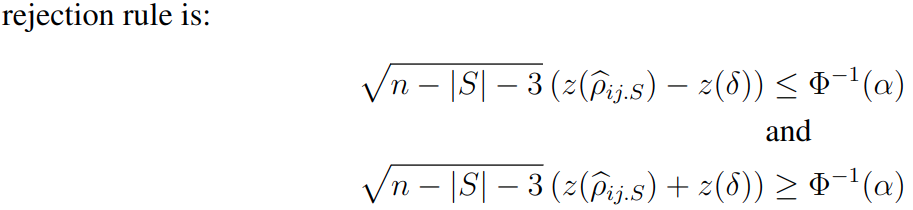
\includegraphics[scale=0.3]{imgs/partial.png}
	\end{figure}
\end{frame}

\begin{frame}{Test Using Expected Conditional Covariance}
	\center{When Gaussianity assumption is not satisfied.}
	\vspace{1em}
	\begin{equation*}
		\begin{split}
			\Psi^*_{ij.S} &= \frac{\mathbb{E}[cov(X_i, X_j | X_S)]}{\sqrt{\mathbb{E}[\sigma^2(X_i \rvert X_S)] \mathbb{E}[\sigma^2(X_j \rvert X_S)]}} \\
			\sqrt{n}(\hat{\Psi}^*_{ij.S} - \Psi^*_{ij.S}) & \sim N(0, \sigma^2_{ij.S}) \\
		\end{split}
	\end{equation*}
	\begin{figure}
		\centering
		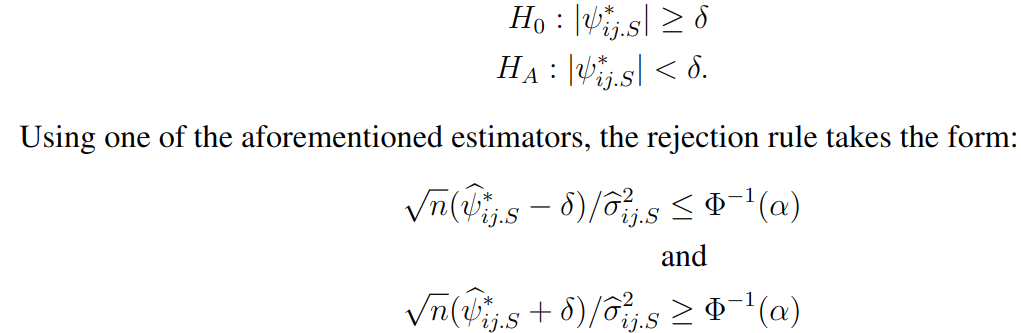
\includegraphics[scale=0.3]{imgs/test2.png}
	\end{figure}
\end{frame}

\begin{frame}{Test Using Odds Ratios}
	In case of mixed variables (continuous and binary), conditional odds ratio.

	\begin{equation*}
		\begin{split}
			\gamma_{ij.S} &= log OR(X_i, X_j \rvert X_S) \\
			\sqrt{n}(\hat{\gamma}_{ij.S} - \gamma_{ij.S}) &\sim N(0, \omega^2_{ij.S}) \\
		\end{split}
	\end{equation*}
	\begin{figure}
		\centering
		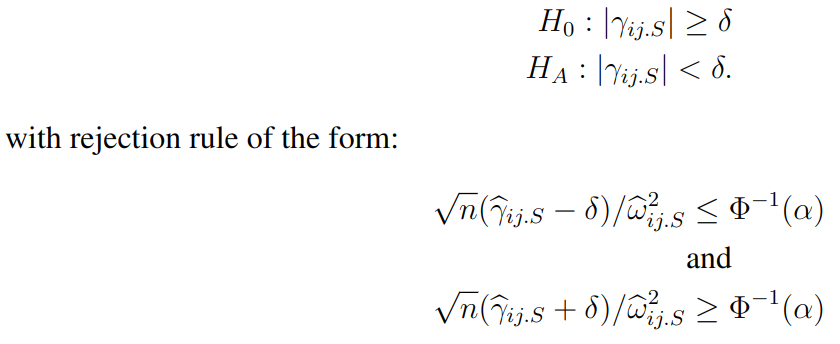
\includegraphics[scale=0.3]{imgs/test3.png}
	\end{figure}
\end{frame}

\begin{frame}{Empirical Results}
	\begin{itemize}
		\item Random graphs on $ 10 $ nodes with an expected degree of $ 7 $.
		\item Very dense graphs, $ < 10 $ missing edges.
		\item Linear data simulation with random ($ [0.5, 1.0] $) parameter value.
		\item Fixed $ \alpha = 0.05 $ for e-PC.
	\end{itemize}
\end{frame}

\begin{frame}{Empirical Results: Recall}
	\begin{figure}
		\centering
		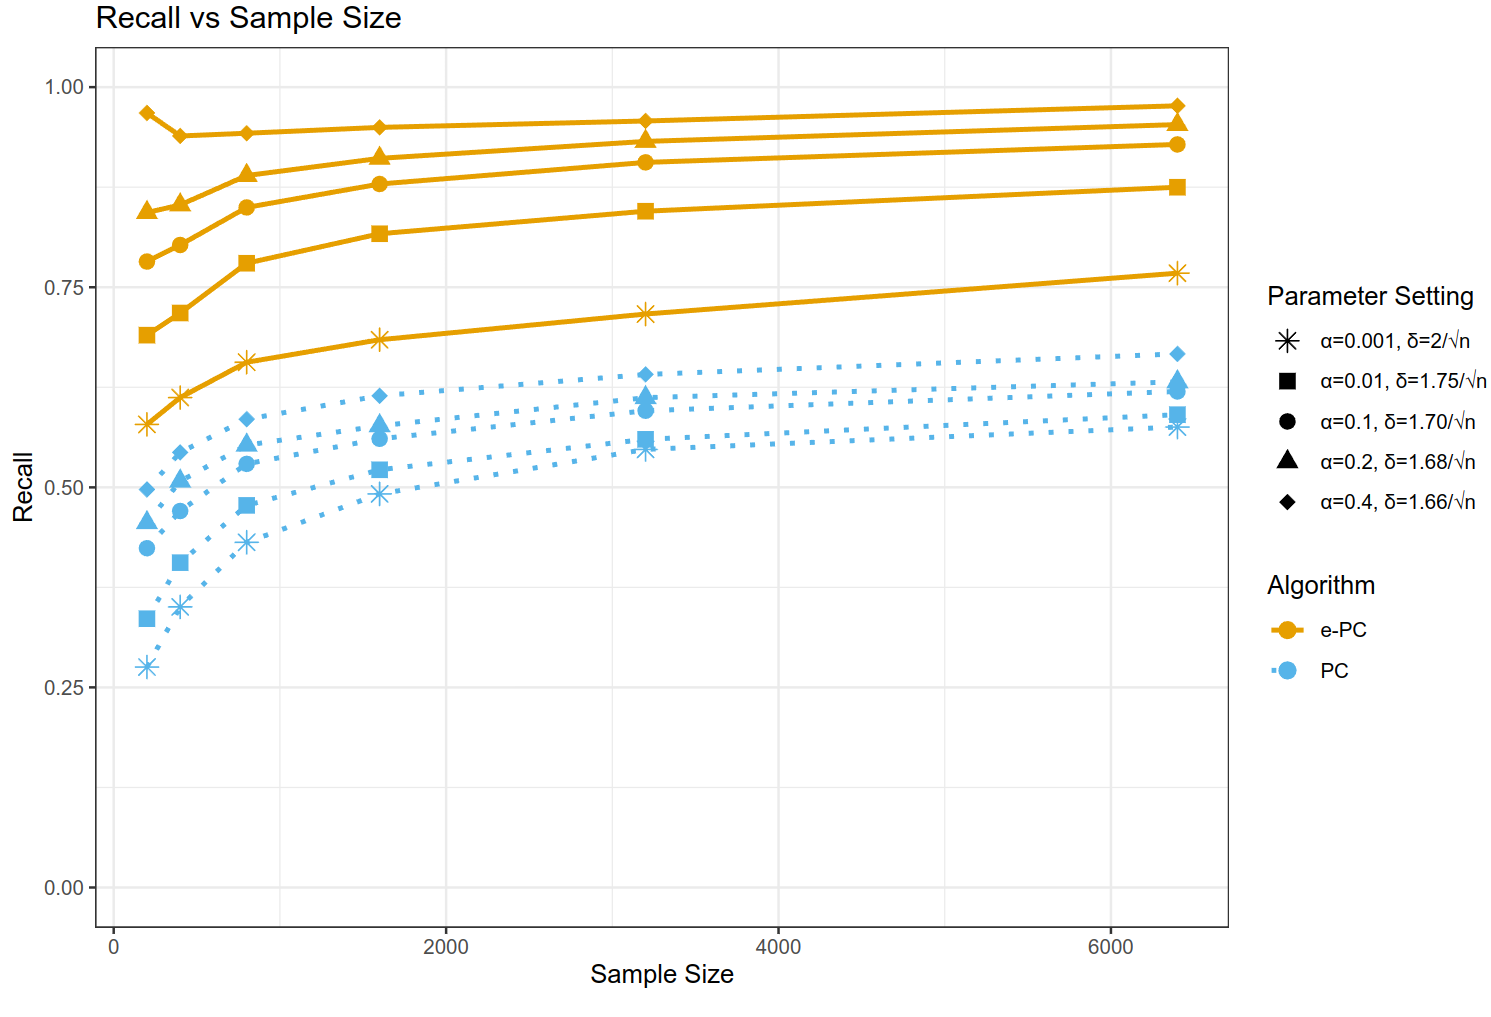
\includegraphics[scale=0.2]{imgs/recall.png}
	\end{figure}
\end{frame}

\begin{frame}{Empirical Results: Precision}
	\begin{figure}
		\centering
		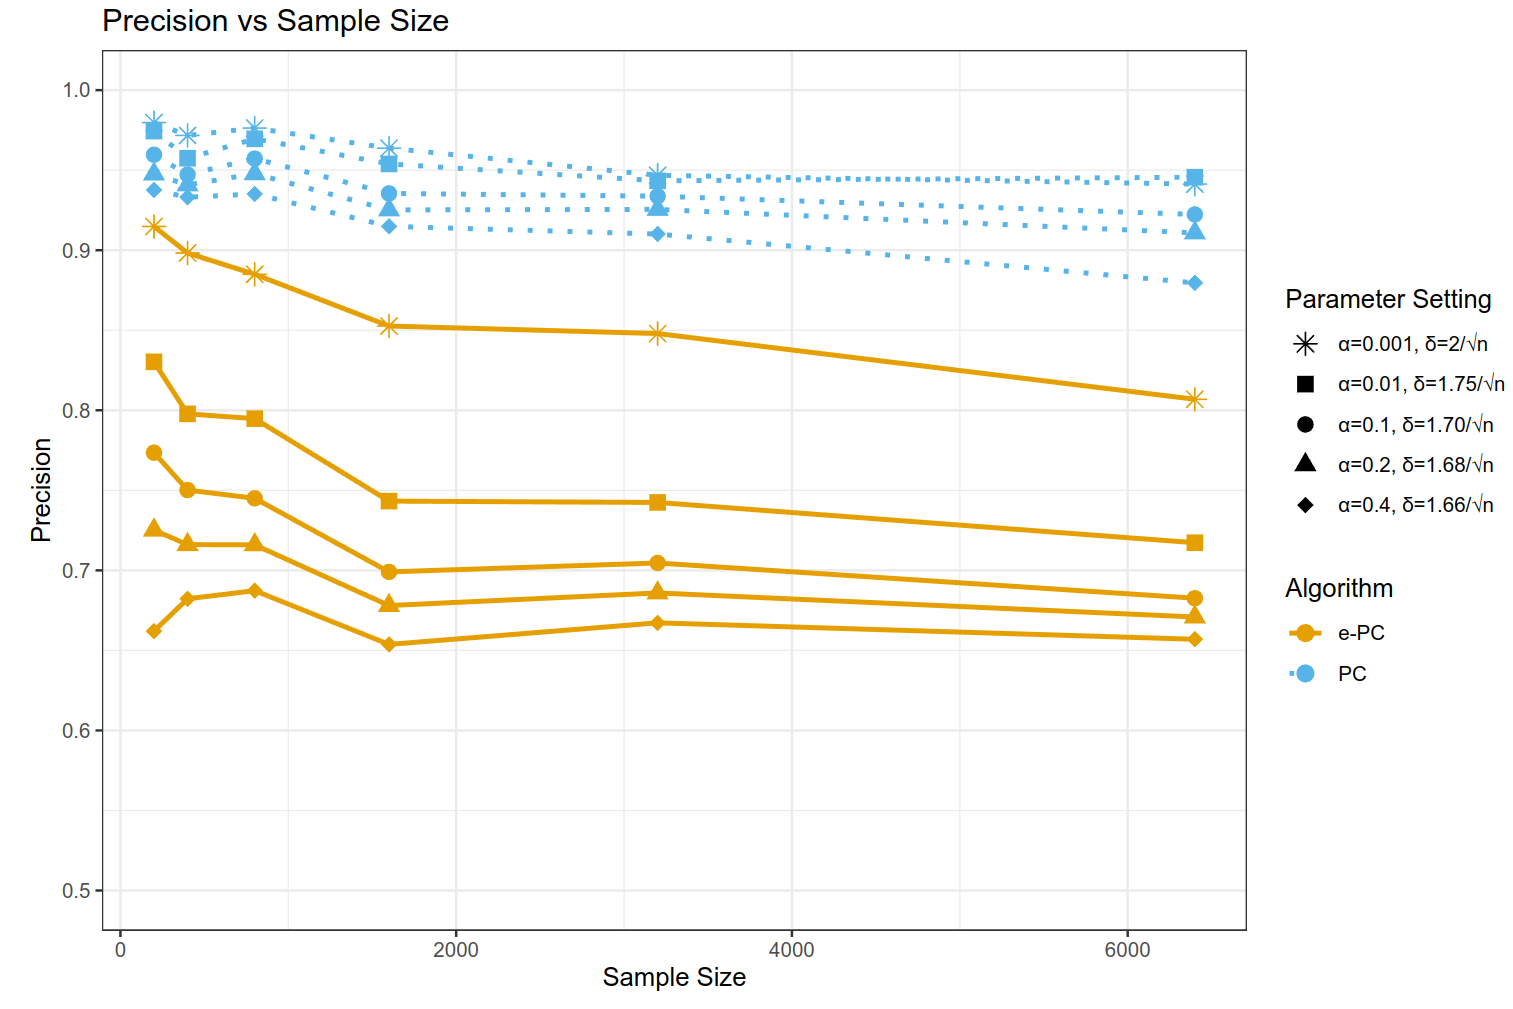
\includegraphics[scale=0.2]{imgs/precision.png}
	\end{figure}
\end{frame}

\begin{frame}{Empirical Analysis: Comparison}
	\begin{figure}
		\centering
		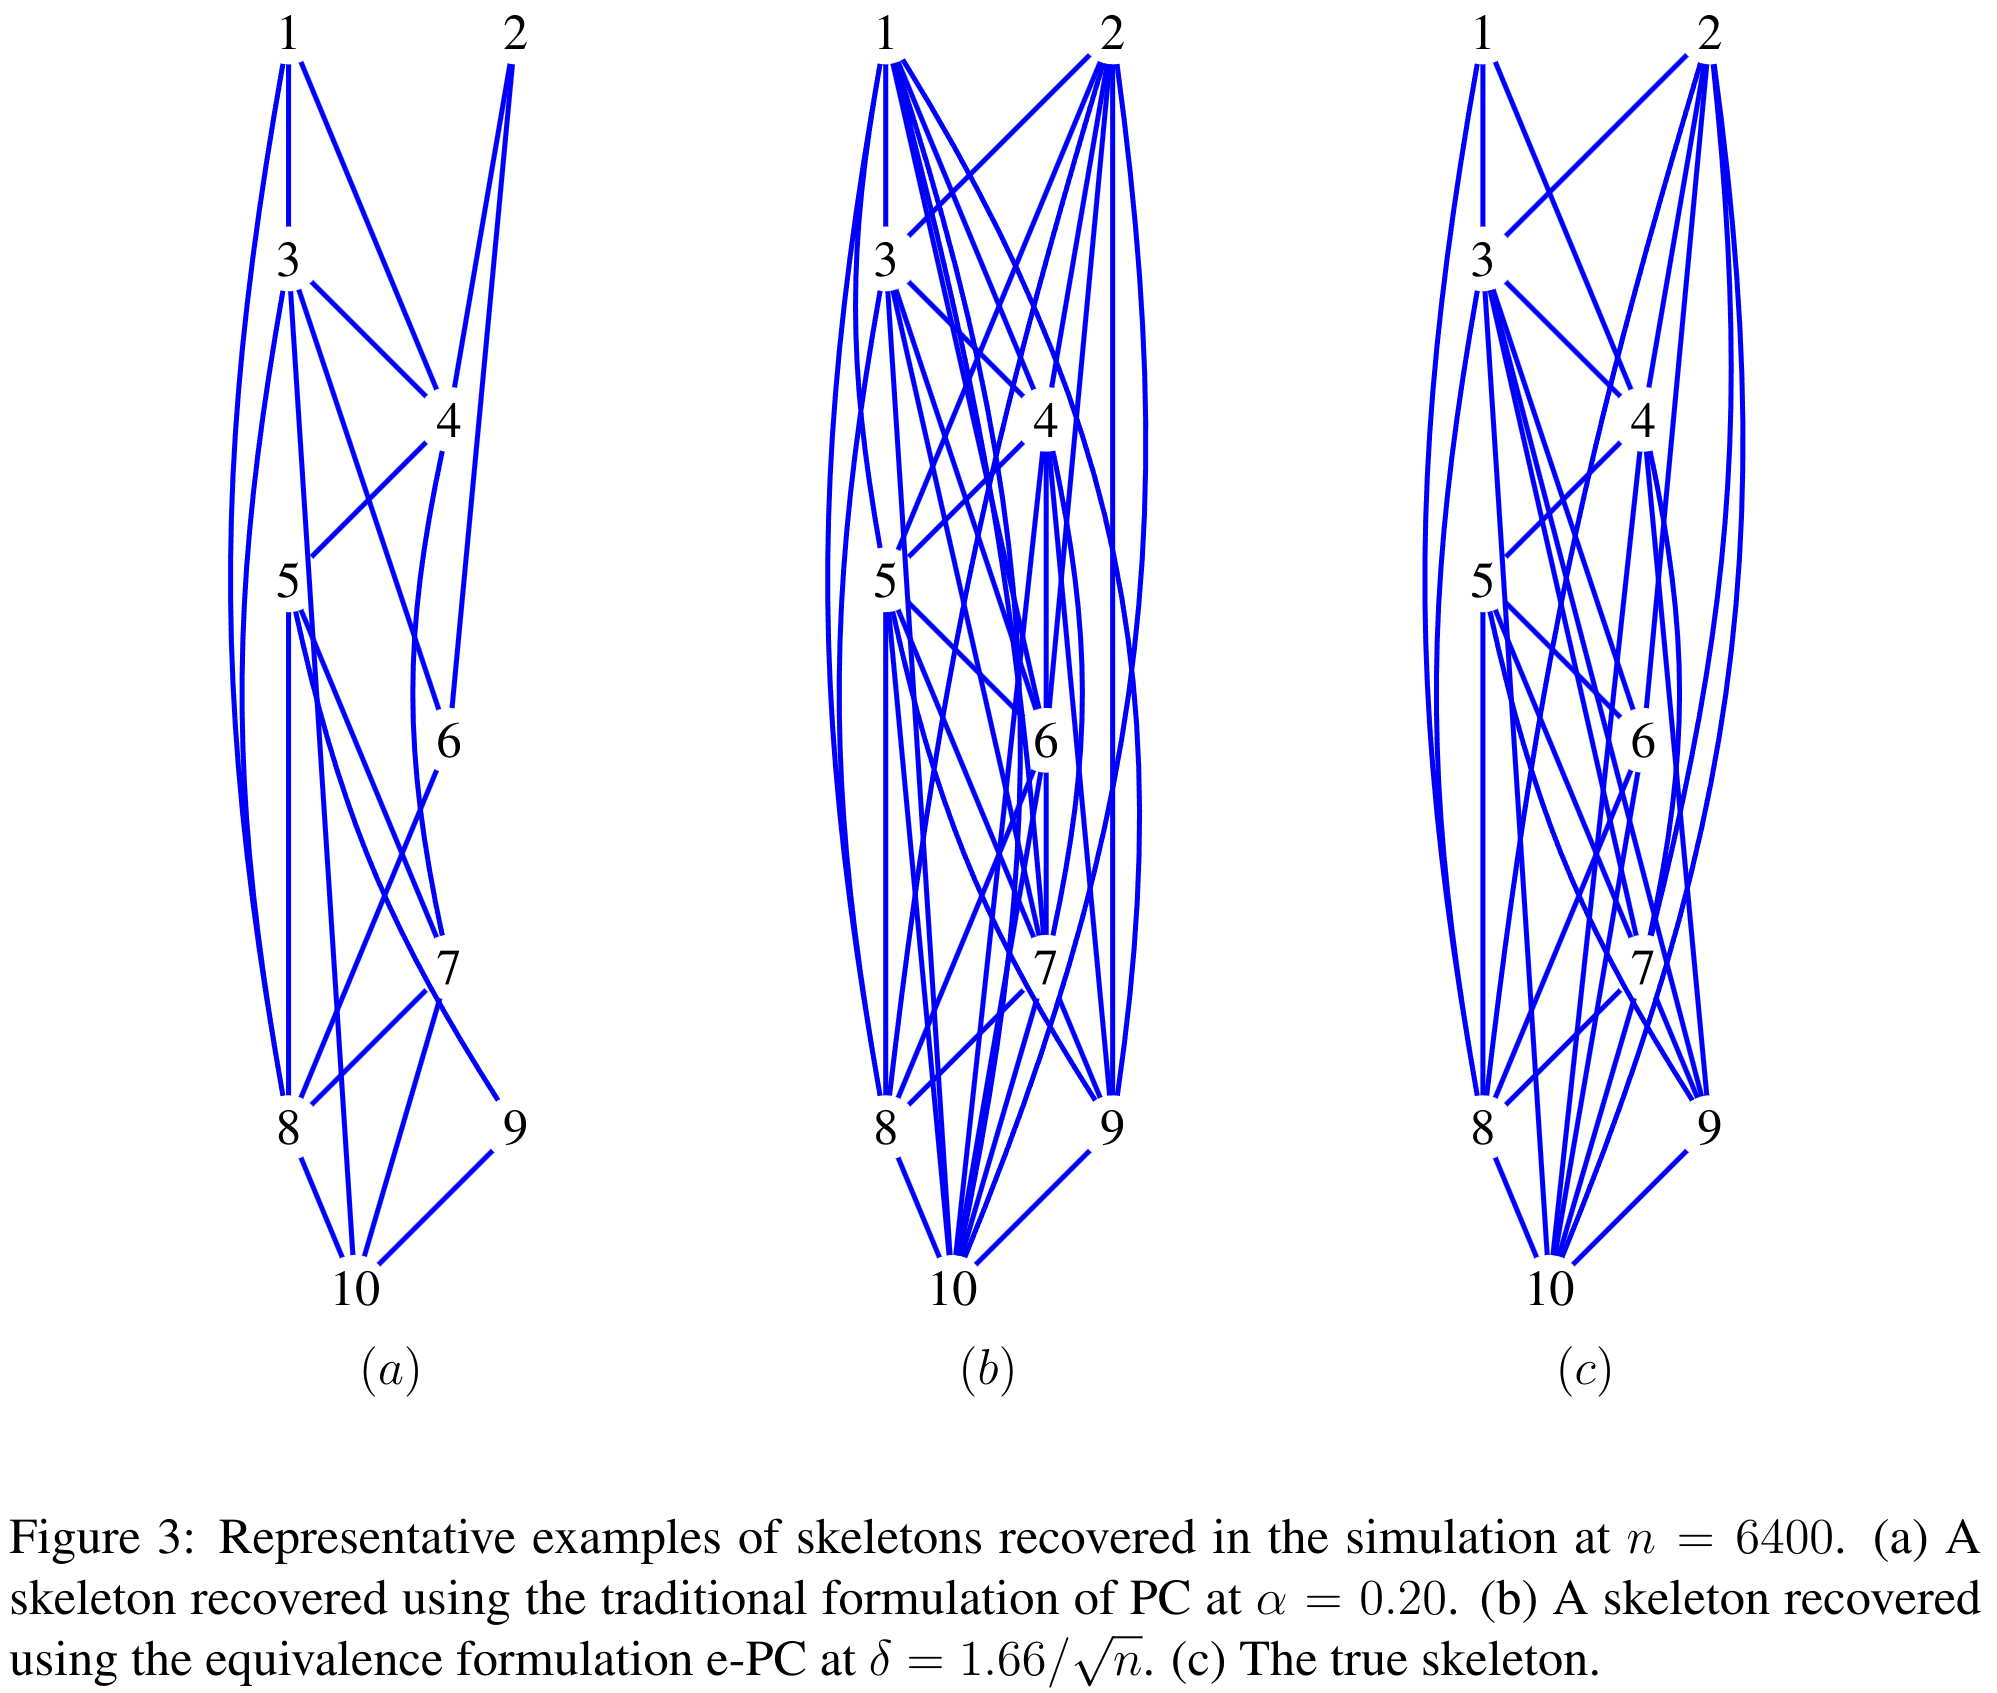
\includegraphics[scale=0.12]{imgs/empirical_compare.png}
	\end{figure}
\end{frame}

\begin{frame}{Empirical Analysis: Effect Estimation}
	\begin{itemize}
		\item Estimate the ATE of $ X_5 $ on $ X_{10} $ where the DAG is topologically ordered: $ X_i < X_{i+1} $.
		\item Learn the CPDAG using PC with partial ordering information:
			$$ (X_1, X_2) < (X_3, X_4, X_5, X_6, X_7) < (X_8, X_9) < X_{10} $$
		\item Gives a set of estimated effects $ \hat{\beta} = (\hat{\beta}^{min}, \cdots, \hat{\beta}^{max}) $
		\item $$ \textnormal{Int-MSE}:  \begin{cases}
				0 & \!\!\!\!\!\!\!\!\!\!\!\!\!\!\!\!\!\!\!\!\!\! \textnormal{if } \hat{\beta}^{min} < \hat{\beta}^{oracle} < \hat{\beta}^{max} \\
				min((\hat{\beta}^{oracle} - \hat{\beta}^{min})^2, (\hat{\beta}^{oracle} - \hat{\beta}^{max})^2) & \textnormal{otherwise} \\
						\end{cases} $$
	\end{itemize}
	\begin{figure}
		\centering
		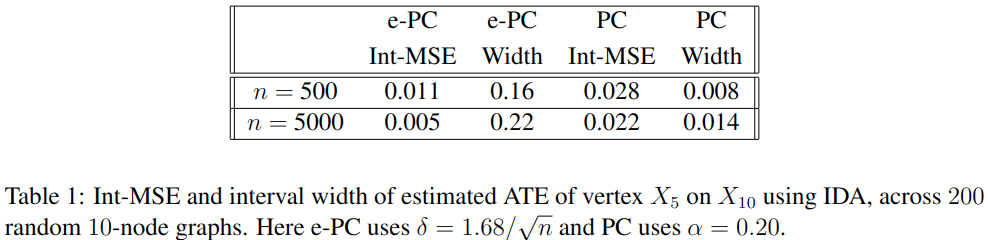
\includegraphics[scale=0.35]{imgs/table1.png}
	\end{figure}
\end{frame}

\begin{frame}{Conclusion}
	\begin{itemize}
		\item Previous approaches to causal discovery has focused on not including false edges.
		\item In context of causal effect estimation, important to have denser models and control for false edge removals.
		\item Paper proposes an inversion of the usual null hypothesis used in CI testing along with tests for it.
		\item This leads to learning denser graphs.
	\end{itemize}
\end{frame}

\end{document}
